\documentclass[aspectratio=169,11pt]{beamer}

% ============================================================
% Theme
% ============================================================
\usetheme{Madrid}
\usecolortheme{seahorse}
\setbeamertemplate{navigation symbols}{}

% ============================================================
% Encoding
% ============================================================
\usepackage[utf8]{inputenc}
\usepackage[T1]{fontenc}
\usepackage{lmodern}

% ============================================================
% Packages
% ============================================================
\usepackage{amsmath,amssymb}
\usepackage{xcolor}
\usepackage{booktabs}
\usepackage{listings}
\usepackage{tikz}
\usetikzlibrary{arrows.meta,positioning,calc,fit}

% ============================================================
% Listings
% ============================================================
\lstset{
	basicstyle=\ttfamily\small,
	frame=single,
	breaklines=true,
	columns=fullflexible,
	showstringspaces=false,
	keywordstyle=\color{blue},
	commentstyle=\color{gray},
	stringstyle=\color{red}
}

% ============================================================
% Title
% ============================================================
\title{Concurrency \& Distributed Systems}
\subtitle{Week 3: Synchronization, Memory Semantics \& Deadlocks\\Day 2 --- Deadlocks, Lock Ordering, and Prevention}
\author{Dr. Mohamad Aoude}
\institute{Lebanese University \\ Faculty of Engineering}
\date{}

% ============================================================
% TikZ Styles
% ============================================================
\tikzset{
	box/.style={draw, rounded corners=2pt, align=center, inner sep=6pt},
	smallbox/.style={draw, rounded corners=2pt, align=center, inner sep=3pt},
	arrow/.style={-Latex, line width=0.8pt},
	dashedarrow/.style={-Latex, dashed, line width=0.8pt},
	tinylabel/.style={font=\scriptsize},
	pill/.style={draw, rounded corners=10pt, inner sep=4pt, align=center}
}

\begin{document}
	
	% ============================================================
	\begin{frame}
		\titlepage
	\end{frame}
	
	% ============================================================
	\section{Week 3 --- Day 2}
	\subsection{Deadlocks, Lock Ordering \& Prevention}
	
	% ============================================================
	\begin{frame}{Day 2 --- From Correctness to Liveness Failure}
		\textbf{Theme:} From safe locking to structural deadlock risk
		
		\bigskip
		
		Today:
		\begin{itemize}
			\item What deadlock is
			\item Why it happens
			\item How opposite lock order creates it
			\item How global ordering prevents it
			\item How to think about debugging it
		\end{itemize}
		
		\bigskip
		\begin{block}{Goal}
			Understand deadlock as a \textbf{liveness failure}: the program is still alive,
			but progress has stopped.
		\end{block}
	\end{frame}
	
	% ============================================================
	\begin{frame}[fragile]{Warm-Up --- Spot the Deadlock}
		\begin{lstlisting}[language=Java]
			// Thread 1
			synchronized(lockA) {
				synchronized(lockB) { }
			}
			
			// Thread 2
			synchronized(lockB) {
				synchronized(lockA) { }
			}
		\end{lstlisting}
		
		\vspace{0.2cm}
		\begin{alertblock}{Question}
			Will this always deadlock? Sometimes? Never? Why?
		\end{alertblock}
		
		\begin{block}{Teaching purpose}
			Start with the puzzle first.  
			Then let the theory explain it.
		\end{block}
	\end{frame}
	
	% ============================================================
	\begin{frame}{Block 1 --- Deadlock Theory}
		\begin{block}{Definition}
			\textbf{Deadlock} occurs when two or more threads are permanently waiting
			for each other’s locks, so none of them can continue.
		\end{block}
		
		\bigskip
		
		\begin{alertblock}{Key idea}
			Deadlock is not about wrong values.  
			It is about \textbf{no progress}.
		\end{alertblock}
	\end{frame}
	
	% ============================================================
	\begin{frame}{How Deadlock Feels in Practice}
		\begin{itemize}
			\item The program may still be running
			\item CPU usage may drop very low
			\item No exception may be thrown
			\item Threads remain blocked forever
		\end{itemize}
		
		\bigskip
		
		\begin{block}{Observation}
			A deadlocked system is not terminated.  
			It is trapped in a waiting structure it cannot escape.
		\end{block}
	\end{frame}
	
	% ============================================================
	\begin{frame}{Deadlock vs Starvation vs Livelock}
		\centering
		\begin{tabular}{@{}llll@{}}
			\toprule
			\textbf{Issue} & \textbf{Threads} & \textbf{Progress} & \textbf{Cause} \\
			\midrule
			Deadlock & Blocked & Never & Circular wait \\
			Starvation & Runnable / waiting often & Never & Unfair scheduling \\
			Livelock & Active & Never & Endless reactions without advance \\
			\bottomrule
		\end{tabular}
		
		\bigskip
		
		\begin{alertblock}{Important}
			These are all liveness failures, but they are not the same problem.
		\end{alertblock}
	\end{frame}
	
	% ============================================================
	\begin{frame}{Coffman Conditions for Deadlock}
		\begin{block}{Deadlock requires four conditions}
			\begin{enumerate}
				\item Mutual exclusion
				\item Hold and wait
				\item No preemption
				\item Circular wait
			\end{enumerate}
		\end{block}
		
		\bigskip
		
		\begin{alertblock}{Important}
			If one of these conditions is broken, deadlock cannot occur.
		\end{alertblock}
	\end{frame}
	
	% ============================================================
	\begin{frame}{Quick Check --- Which Conditions Can We Break?}
		\begin{block}{Practical question}
			Which Coffman conditions can we realistically design against in Java?
		\end{block}
		
		\bigskip
		
		\begin{itemize}
			\item Mutual exclusion? Usually no --- locks depend on it
			\item Hold and wait? Sometimes yes
			\item No preemption? Usually no for intrinsic monitors
			\item Circular wait? Yes --- this is the main design lever
		\end{itemize}
		
		\bigskip
		
		\begin{alertblock}{Takeaway}
			The most practical prevention strategy is often: \textbf{break circular wait}.
		\end{alertblock}
	\end{frame}
	
	% ============================================================
	\begin{frame}{Condition 1 --- Mutual Exclusion}
		\begin{block}{Meaning}
			At least one resource must be held in an exclusive way.
		\end{block}
		
		\bigskip
		
		\begin{itemize}
			\item A Java monitor can be owned by only one thread at a time
			\item If a resource were freely shareable, deadlock would not arise on that resource
		\end{itemize}
		
		\bigskip
		
		\begin{alertblock}{Interpretation}
			The same exclusivity that protects correctness can create deadlock risk.
		\end{alertblock}
	\end{frame}
	
	% ============================================================
	\begin{frame}{Condition 2 --- Hold and Wait}
		\begin{block}{Meaning}
			A thread holds one lock while waiting to acquire another.
		\end{block}
		
		\bigskip
		
		\begin{itemize}
			\item Thread 1 holds lock A and waits for lock B
			\item Thread 2 holds lock B and waits for lock A
		\end{itemize}
		
		\bigskip
		
		\begin{alertblock}{Interpretation}
			A thread is not releasing what it already owns before asking for more.
		\end{alertblock}
	\end{frame}
	
	% ============================================================
	\begin{frame}{Condition 3 --- No Preemption}
		\begin{block}{Meaning}
			A lock cannot be forcibly taken away from a thread.
		\end{block}
		
		\bigskip
		
		\begin{itemize}
			\item Java does not let one thread steal another thread’s monitor
			\item The owner must release the lock voluntarily
		\end{itemize}
		
		\bigskip
		
		\begin{alertblock}{Interpretation}
			If locks could be revoked automatically, some deadlocks could be broken by force.
		\end{alertblock}
	\end{frame}
	
	% ============================================================
	\begin{frame}{Condition 4 --- Circular Wait}
		\begin{block}{Meaning}
			A cycle exists in the waiting relationships.
		\end{block}
		
		\bigskip
		
		\[
		T_1 \rightarrow T_2 \rightarrow T_3 \rightarrow \dots \rightarrow T_1
		\]
		
		\bigskip
		
		\begin{alertblock}{Analogy}
			Think of two cars facing each other on a narrow bridge.  
			Each waits for the other to move first. Neither can progress.
		\end{alertblock}
	\end{frame}
	
	% ============================================================
	\begin{frame}{The Most Important Condition to Watch}
		\begin{block}{Practical teaching focus}
			All four conditions matter, but \textbf{circular wait} is the clearest structural pattern.
		\end{block}
		
		\bigskip
		
		\begin{itemize}
			\item Mutual exclusion is usually intentional
			\item No preemption is built into monitor behavior
			\item Hold-and-wait appears naturally in nested locking
			\item Circular wait is the pattern we can design against
		\end{itemize}
		
		\bigskip
		
		\centering
		\Large Prevent circular wait \(\Rightarrow\) prevent deadlock
	\end{frame}
	
	% ============================================================
	\begin{frame}{Block 2 --- Creating Deadlock}
		\begin{block}{Demo idea}
			Two locks are acquired in opposite order by two threads.
		\end{block}
		
		\bigskip
		
		\begin{itemize}
			\item Thread 1 acquires lock A, then tries for lock B
			\item Thread 2 acquires lock B, then tries for lock A
		\end{itemize}
		
		\bigskip
		
		\begin{alertblock}{Expected result}
			The program freezes because each thread waits for the other forever.
		\end{alertblock}
	\end{frame}
	
	% ============================================================
	\begin{frame}[fragile]{Deadlock Demo --- Thread 1}
		\begin{lstlisting}[language=Java]
			synchronized(lockA) {
				System.out.println("Thread 1 acquired lockA");
				
				synchronized(lockB) {
					System.out.println("Thread 1 acquired lockB");
				}
			}
		\end{lstlisting}
		
		\vspace{0.3cm}
		\begin{block}{Order}
			Thread 1 acquires \texttt{lockA} first, then \texttt{lockB}.
		\end{block}
		
		\begin{alertblock}{Reentrancy note}
			Java locks are reentrant: a thread may re-acquire a lock it already holds.  
			That prevents self-deadlock, but it does not prevent inter-thread cycles.
		\end{alertblock}
	\end{frame}
	
	% ============================================================
	\begin{frame}[fragile]{Deadlock Demo --- Thread 2}
		\begin{lstlisting}[language=Java]
			synchronized(lockB) {
				System.out.println("Thread 2 acquired lockB");
				
				synchronized(lockA) {
					System.out.println("Thread 2 acquired lockA");
				}
			}
		\end{lstlisting}
		
		\vspace{0.3cm}
		\begin{block}{Order}
			Thread 2 acquires \texttt{lockB} first, then \texttt{lockA}.
		\end{block}
	\end{frame}
	

	
	% ============================================================
\begin{frame}{Execution Trace --- How Deadlock Forms}
	
	\begin{center}
		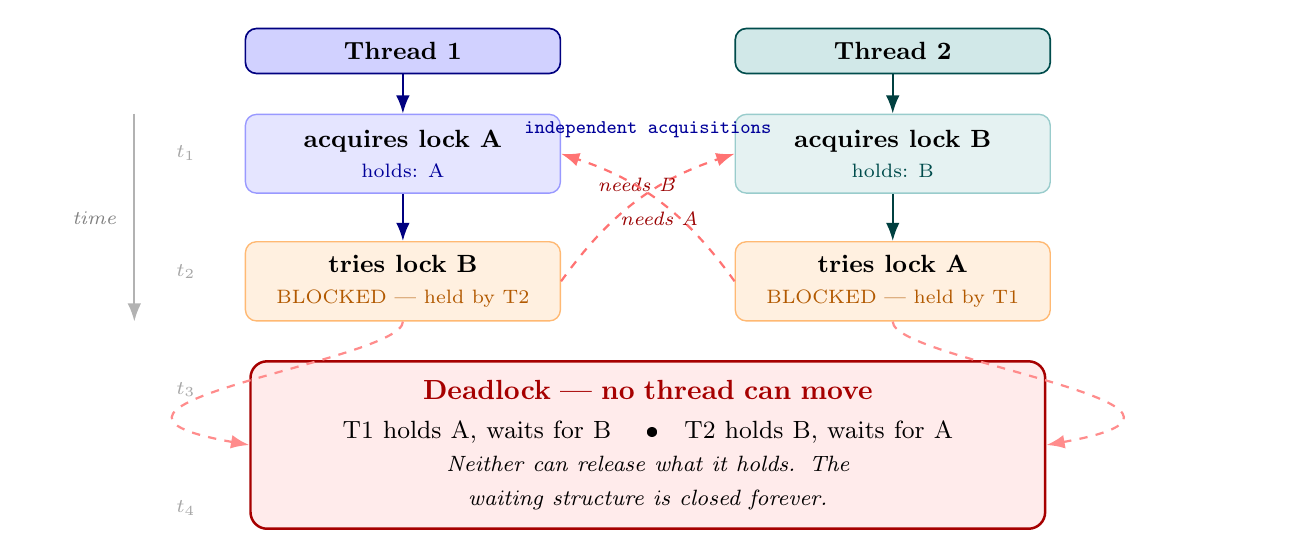
\begin{tikzpicture}[
			stepbox/.style={draw, rounded corners=4pt, align=center,
				inner sep=5pt, font=\small},
			stepnum/.style={font=\scriptsize\bfseries, text=gray!70},
			]
			
			%% -- Column headers
			\node[stepbox, fill=blue!18, draw=blue!50!black, line width=0.6pt,
			minimum width=4.0cm, font=\small\bfseries] (h1)
			{Thread 1};
			
			\node[stepbox, fill=teal!18, draw=teal!60!black, line width=0.6pt,
			minimum width=4.0cm, font=\small\bfseries,
			right=22mm of h1] (h2)
			{Thread 2};
			
			%% -- Step numbers (left margin)
			\node[stepnum, left=5mm of h1, yshift=-13mm] {$t_1$};
			\node[stepnum, left=5mm of h1, yshift=-28mm] {$t_2$};
			\node[stepnum, left=5mm of h1, yshift=-43mm] {$t_3$};
			\node[stepnum, left=5mm of h1, yshift=-58mm] {$t_4$};
			
			%% -- t1: Thread 1 acquires lock A
			\node[stepbox, fill=blue!10, draw=blue!40, line width=0.5pt,
			minimum width=4.0cm, minimum height=1.0cm,
			below=5mm of h1] (s1)
			{\textbf{acquires lock A}\\
				\scriptsize\textcolor{blue!60!black}{holds: A}};
			
			%% -- t2: Thread 2 acquires lock B
			\node[stepbox, fill=teal!10, draw=teal!40, line width=0.5pt,
			minimum width=4.0cm, minimum height=1.0cm,
			below=5mm of h2] (s2)
			{\textbf{acquires lock B}\\
				\scriptsize\textcolor{teal!60!black}{holds: B}};
			
			%% -- t3: Thread 1 blocked on B
			\node[stepbox, fill=orange!12, draw=orange!55, line width=0.5pt,
			minimum width=4.0cm, minimum height=1.0cm,
			below=6mm of s1] (s3)
			{\textbf{tries lock B}\\
				\scriptsize\textcolor{orange!70!black}{BLOCKED --- held by T2}};
			
			%% -- t4: Thread 2 blocked on A
			\node[stepbox, fill=orange!12, draw=orange!55, line width=0.5pt,
			minimum width=4.0cm, minimum height=1.0cm,
			below=6mm of s2] (s4)
			{\textbf{tries lock A}\\
				\scriptsize\textcolor{orange!70!black}{BLOCKED --- held by T1}};
			
			%% -- Thread flow arrows
			\draw[arrow, blue!50!black]  (h1) -- (s1);
			\draw[arrow, blue!50!black]  (s1) -- (s3);
			\draw[arrow, teal!50!black]  (h2) -- (s2);
			\draw[arrow, teal!50!black]  (s2) -- (s4);
			
%% -- Time axis (left) — anchored to h1.west for true vertical
\coordinate (axistop) at ([xshift=-14mm] h1.west |- s1.north);
\coordinate (axisbot) at ([xshift=-14mm] h1.west |- s3.south);
\draw[arrow, gray!60] (axistop) -- (axisbot)
node[midway, left=1mm, font=\scriptsize\itshape, text=gray] {time};
			
			%% -- Centre: lock state annotations
			\coordinate (midAB) at ($(h1.east)!0.5!(h2.west)$);
			
			\node[font=\scriptsize\ttfamily, text=blue!60!black, align=center]
			at ($(s1)!0.5!(s2)+(0,3mm)$) {independent acquisitions};
			
			%% -- Blocking cross-arrows (the cycle)
			\draw[dashedarrow, red!55, line width=0.8pt]
			(s3.east) to[bend left=18]
			node[above, font=\scriptsize\itshape, text=red!60!black] {needs B}
			(s2.west);
			
			\draw[dashedarrow, red!55, line width=0.8pt]
			(s4.west) to[bend right=18]
			node[below, font=\scriptsize\itshape, text=red!60!black] {needs A}
			(s1.east);
			
			%% -- Deadlock result box
			\node[draw=red!65!black, fill=red!8, rounded corners=6pt,
			text width=9.6cm, align=center,
			inner sep=7pt, line width=0.9pt,
			below=10mm of $(s3)!0.5!(s4)$] (dead)
			{
				\textcolor{red!65!black}{\textbf{Deadlock --- no thread can move}}\\[3pt]
				\small
				T1 holds A, waits for B \quad\textbullet\quad T2 holds B, waits for A\\
				\footnotesize\itshape
				Neither can release what it holds. The waiting structure is closed forever.
			};
			
			\draw[dashedarrow, red!45] (s3.south) .. controls +(0,-5mm) and +(-28mm,5mm) .. (dead.west);
			\draw[dashedarrow, red!45] (s4.south) .. controls +(0,-5mm) and +(28mm,5mm)  .. (dead.east);
			
		\end{tikzpicture}
	\end{center}
	
\end{frame}
	
\begin{frame}{Deadlock --- Resource Dependency Graph}
	
	\begin{center}
		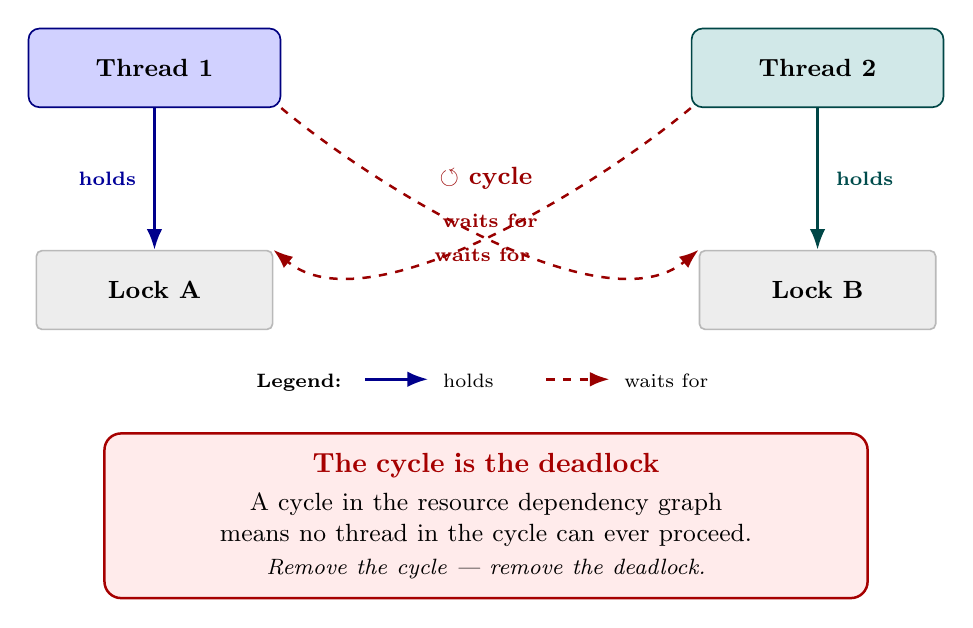
\begin{tikzpicture}[
			threadbox/.style={draw, rounded corners=4pt, align=center,
				inner sep=7pt, font=\small},
			lockbox/.style={draw, rounded corners=2pt, align=center,
				inner sep=7pt, font=\small},
			]
			
			%% -- Thread nodes
			\node[threadbox, fill=blue!18, draw=blue!50!black, line width=0.6pt,
			minimum width=3.2cm, minimum height=1.0cm] (t1)
			{\textbf{Thread 1}};
			
			\node[threadbox, fill=teal!18, draw=teal!55!black, line width=0.6pt,
			minimum width=3.2cm, minimum height=1.0cm,
			right=52mm of t1] (t2)
			{\textbf{Thread 2}};
			
			%% -- Lock nodes (below threads, centred between them)
			\node[lockbox, fill=gray!14, draw=gray!55, line width=0.6pt,
			minimum width=3.0cm, minimum height=1.0cm,
			below=18mm of t1] (la)
			{\textbf{Lock A}};
			
			\node[lockbox, fill=gray!14, draw=gray!55, line width=0.6pt,
			minimum width=3.0cm, minimum height=1.0cm,
			below=18mm of t2] (lb)
			{\textbf{Lock B}};
			
			%% -- HOLDS edges (solid, colored)
			\draw[arrow, blue!55!black, line width=1.0pt]
			(t1.south) -- (la.north)
			node[midway, left=1mm, font=\scriptsize\bfseries, text=blue!60!black]
			{holds};
			
			\draw[arrow, teal!55!black, line width=1.0pt]
			(t2.south) -- (lb.north)
			node[midway, right=1mm, font=\scriptsize\bfseries, text=teal!60!black]
			{holds};
			
			%% -- WAITS FOR edges (dashed red, crossing)
			\draw[dashedarrow, red!60!black, line width=0.9pt]
			(t1.south east) .. controls +(12mm,-10mm) and +(-12mm,-10mm) .. (lb.north west)
			node[midway, above, font=\scriptsize\bfseries, text=red!60!black]
			{waits for};
			
			\draw[dashedarrow, red!60!black, line width=0.9pt]
			(t2.south west) .. controls +(-12mm,-10mm) and +(12mm,-10mm) .. (la.north east)
			node[midway, below, font=\scriptsize\bfseries, text=red!60!black]
			{waits for};
			
			%% -- Cycle label in the centre
			\node[font=\small\bfseries, text=red!60!black, align=center]
			at ($(t1.east)!0.5!(t2.west) + (0,-14mm)$)
			{\textcolor{red!60!black}{$\circlearrowleft$ cycle}};
			
			%% -- Legend
			\node[font=\scriptsize, align=left,
			below=4mm of $(la.south)!0.5!(lb.south)$] (leg)
			{
				\textbf{Legend:}\quad
				\tikz[baseline=-1mm]{\draw[arrow, blue!55!black, line width=1.0pt] (0,0) -- (8mm,0);}
				\;\scriptsize holds \qquad
				\tikz[baseline=-1mm]{\draw[dashedarrow, red!60!black, line width=0.9pt] (0,0) -- (8mm,0);}
				\;\scriptsize waits for
			};
			
			%% -- Deadlock verdict box
			\node[draw=red!65!black, fill=red!8, rounded corners=6pt,
			text width=9.2cm, align=center,
			inner sep=7pt, line width=0.9pt,
			below=4mm of leg] (dead)
			{
				\textcolor{red!65!black}{\textbf{The cycle is the deadlock}}\\[3pt]
				\small
				A cycle in the resource dependency graph means
				no thread in the cycle can ever proceed.\\
				\footnotesize\itshape
				Remove the cycle --- remove the deadlock.
			};
			
		\end{tikzpicture}
	\end{center}

\end{frame}
	

	
	% ============================================================
	\begin{frame}{Why It Never Progresses}
		\begin{enumerate}
			\item Thread 1 cannot proceed until Thread 2 releases lock B
			\item Thread 2 cannot proceed until Thread 1 releases lock A
			\item Neither thread can release its first lock because each is blocked waiting for the second
		\end{enumerate}
		
		\bigskip
		
		\begin{alertblock}{Conclusion}
			No thread can move first.  
			The waiting structure is closed.
		\end{alertblock}
	\end{frame}
	

	
	% ============================================================
	\begin{frame}{Block 3 --- Lock Ordering Principle}
		\begin{block}{Rule}
			If all threads acquire locks in the same global order,
			deadlock cannot occur.
		\end{block}
		
		\bigskip
		
		\begin{alertblock}{Core design idea}
			A consistent lock order destroys the possibility of circular wait.
		\end{alertblock}
	\end{frame}
	
\begin{frame}[fragile]{Deadlock-Free Rewrite --- Consistent Lock Order}
	
	\begin{columns}[T]
		
		%% -- Left column: code
		\begin{column}{0.44\textwidth}
			\begin{block}{Both threads use the same order}
				\begin{lstlisting}[language=Java]
// Thread 1
synchronized(lockA) {
	synchronized(lockB) {
		// critical section
	}
}
// Thread 2
synchronized(lockA) {
	synchronized(lockB) {
			// critical section
	}
}
				\end{lstlisting}
			\end{block}
		\end{column}
		
		%% -- Right column: diagram + reasoning
		\begin{column}{0.52\textwidth}
			\begin{center}
				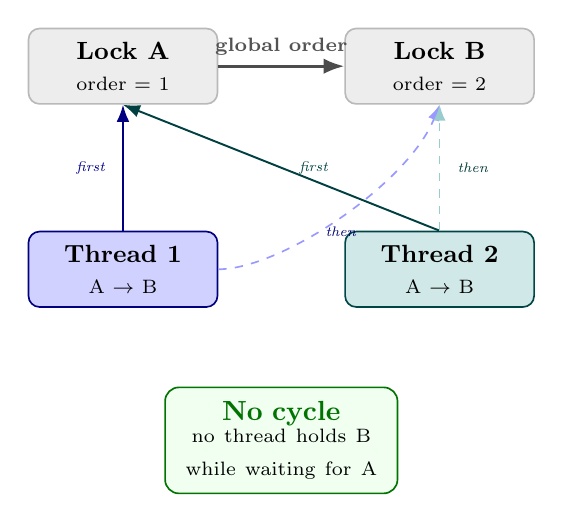
\begin{tikzpicture}[
					stepbox/.style={draw, rounded corners=4pt, align=center,
						inner sep=5pt, font=\small},
					]
					
					%% -- Lock order bar
					\node[stepbox, fill=gray!14, draw=gray!55, line width=0.6pt,
					minimum width=2.4cm, minimum height=0.9cm] (la)
					{\textbf{Lock A}\\\scriptsize order = 1};
					
					\node[stepbox, fill=gray!14, draw=gray!55, line width=0.6pt,
					minimum width=2.4cm, minimum height=0.9cm,
					right=16mm of la] (lb)
					{\textbf{Lock B}\\\scriptsize order = 2};
					
					\draw[arrow, gray!60!black, line width=1.0pt]
					(la.east) -- (lb.west)
					node[midway, above, font=\scriptsize\bfseries, text=gray!65!black]
					{global order};
					
					%% -- Thread 1
					\node[stepbox, fill=blue!18, draw=blue!50!black, line width=0.6pt,
					minimum width=2.4cm, minimum height=0.9cm,
					below=16mm of la] (t1)
					{\textbf{Thread 1}\\\scriptsize A \(\rightarrow\) B};
					
					%% -- Thread 2
					\node[stepbox, fill=teal!18, draw=teal!55!black, line width=0.6pt,
					minimum width=2.4cm, minimum height=0.9cm,
					below=16mm of lb] (t2)
					{\textbf{Thread 2}\\\scriptsize A \(\rightarrow\) B};
					
					%% -- Both point to Lock A first
					\draw[arrow, blue!50!black, line width=0.7pt]
					(t1.north) -- (la.south)
					node[midway, left=1mm, font=\tiny\itshape, text=blue!55!black]
					{first};
					
					\draw[arrow, teal!50!black, line width=0.7pt]
					(t2.north) -- (la.south)
					node[midway, right=1mm, font=\tiny\itshape, text=teal!55!black]
					{first};
					
					%% -- Then to Lock B
					\draw[dashedarrow, blue!40, line width=0.6pt]
					(t1.east) .. controls +(8mm,0mm) and +(-4mm,-10mm) .. (lb.south)
					node[midway, below, font=\tiny\itshape, text=blue!45!black]
					{then};
					
					\draw[dashedarrow, teal!40, line width=0.6pt]
					(t2.north) -- (lb.south)
					node[midway, right=1mm, font=\tiny\itshape, text=teal!45!black]
					{then};
					
					%% -- No cycle badge
					\node[draw=green!45!black, fill=green!6, rounded corners=5pt,
					text width=2.6cm, align=center, inner sep=5pt, line width=0.6pt,
					below=10mm of $(t1.south)!0.5!(t2.south)$] (nocycle)
					{
						\textcolor{green!45!black}{\textbf{No cycle}}\\
						\scriptsize no thread holds B\\while waiting for A
					};
					
				\end{tikzpicture}
			\end{center}
			
			\vspace{2mm}
			\begin{itemize}\small
				\item One thread may \textbf{wait} for lock A
				\item No thread holds B while waiting for A
				\item Therefore the \textbf{cycle cannot form}
			\end{itemize}
		\end{column}
		
	\end{columns}
	
\end{frame}
	
	% ============================================================
\begin{frame}{Why Lock Ordering Works}
	
	\begin{center}
		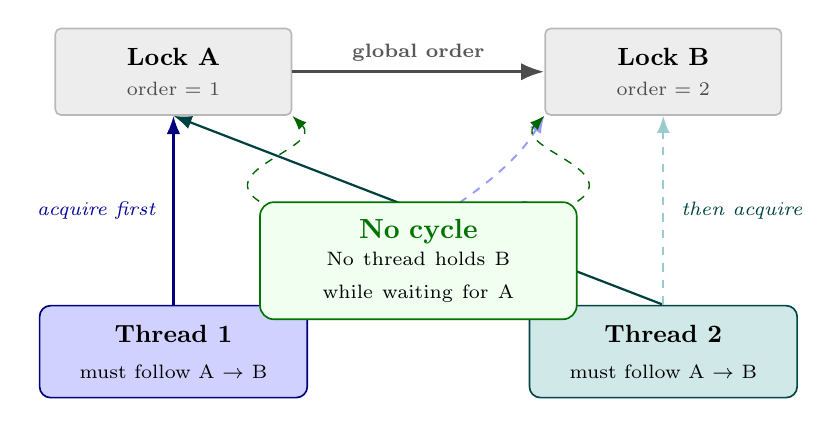
\begin{tikzpicture}[
			threadbox/.style={draw, rounded corners=4pt, align=center,
				inner sep=7pt, font=\small},
			lockbox/.style={draw, rounded corners=2pt, align=center,
				inner sep=7pt, font=\small},
			]
			
			%% -- Global order arrow + lock nodes (top row)
			\node[lockbox, fill=gray!14, draw=gray!55, line width=0.6pt,
			minimum width=3.0cm, minimum height=1.0cm] (la)
			{\textbf{Lock A}\\\scriptsize\textcolor{gray!60!black}{order = 1}};
			
			\node[lockbox, fill=gray!14, draw=gray!55, line width=0.6pt,
			minimum width=3.0cm, minimum height=1.0cm,
			right=32mm of la] (lb)
			{\textbf{Lock B}\\\scriptsize\textcolor{gray!60!black}{order = 2}};
			
			\draw[arrow, gray!60!black, line width=1.2pt]
			(la.east) -- (lb.west)
			node[midway, above, font=\scriptsize\bfseries, text=gray!70!black]
			{global order};
			
			%% -- Thread nodes (below locks)
			\node[threadbox, fill=blue!18, draw=blue!50!black, line width=0.6pt,
			minimum width=3.4cm, minimum height=1.1cm,
			below=24mm of la] (t1)
			{
				\textbf{Thread 1}\\[2pt]
				\scriptsize must follow A \(\rightarrow\) B
			};
			
			\node[threadbox, fill=teal!18, draw=teal!55!black, line width=0.6pt,
			minimum width=3.4cm, minimum height=1.1cm,
			below=24mm of lb] (t2)
			{
				\textbf{Thread 2}\\[2pt]
				\scriptsize must follow A \(\rightarrow\) B
			};
			
			%% -- Both threads point to Lock A first (step 1)
			\draw[arrow, blue!50!black, line width=0.8pt]
			(t1.north) -- (la.south)
			node[midway, left=1mm, font=\scriptsize\itshape, text=blue!60!black]
			{acquire first};
			
			\draw[arrow, teal!50!black, line width=0.8pt]
			(t2.north) -- (la.south)
			node[midway, right=1mm, font=\scriptsize\itshape, text=teal!60!black]
			{acquire first};
			
			%% -- Then both proceed to Lock B (step 2)
			\draw[dashedarrow, blue!40, line width=0.7pt]
			(t1.north east) .. controls +(10mm,8mm) and +(-6mm,-10mm) .. (lb.south west)
			node[midway, below, font=\scriptsize\itshape, text=blue!50!black]
			{then acquire};
			
			\draw[dashedarrow, teal!40, line width=0.7pt]
			(t2.north) -- (lb.south)
			node[midway, right=1mm, font=\scriptsize\itshape, text=teal!50!black]
			{then acquire};
			
			%% -- "No cycle possible" annotation in centre
			\node[draw=green!45!black, fill=green!6, rounded corners=5pt,
			text width=3.6cm, align=center,
			inner sep=6pt, line width=0.6pt]
			at ($(la.east)!0.5!(lb.west) + (0,-24mm)$) (nocycle)
			{
				\textcolor{green!45!black}{\textbf{No cycle}}\\[2pt]
				\scriptsize
				No thread holds B\\
				while waiting for A
			};
			
			%% -- Why no cycle: short explanation arrows
			\draw[dashedarrow, green!40!black, line width=0.5pt]
			(nocycle.north west) .. controls +(-6mm,4mm) and +(4mm,-4mm) .. (la.south east);
			\draw[dashedarrow, green!40!black, line width=0.5pt]
			(nocycle.north east) .. controls +(6mm,4mm) and +(-4mm,-4mm) .. (lb.south west);
			
		\end{tikzpicture}
	\end{center}
	
	\vspace{0.1cm}
	\begin{alertblock}{Key logic}
		If every thread acquires locks in the same global order,
		no thread can hold a higher-order lock while waiting for a lower-order one ---
		the waiting graph \textbf{cannot contain a cycle}.
	\end{alertblock}
	
\end{frame}
	
	% ============================================================
	\begin{frame}{Lock Hierarchy}
		\begin{block}{Concept}
			A \textbf{lock hierarchy} is a fixed global ordering of locks.
		\end{block}
		
		\bigskip
		
		Example:
		\[
		lockA \;<\; lockB \;<\; lockC
		\]
		
		\bigskip
		
		\begin{itemize}
			\item Threads may acquire \(lockA\) then \(lockB\)
			\item Threads may acquire \(lockB\) then \(lockC\)
			\item Threads must never go backward in the hierarchy
		\end{itemize}
		
		\bigskip
		
		\begin{alertblock}{Edge case}
			If locks are chosen dynamically at runtime, we need a consistent rule
			for ordering them, not just a visual hierarchy in the source code.
		\end{alertblock}
	\end{frame}
	
	% ============================================================
	\begin{frame}[fragile]{Dynamic Lock Ordering Example --- Transfer}
		\begin{lstlisting}[language=Java]
			void transfer(Account from, Account to, int amount) {
				synchronized(from) {
					synchronized(to) {
						// move money
					}
				}
			}
		\end{lstlisting}
		
		\vspace{0.3cm}
		
		\begin{alertblock}{Subtle bug}
			If one thread transfers A \(\rightarrow\) B and another transfers B \(\rightarrow\) A,
			the order is reversed dynamically.
		\end{alertblock}
	\end{frame}
	
	% ============================================================
	\begin{frame}{How to Fix Dynamic Lock Ordering}
		\begin{block}{Concrete strategy}
			Order locks by a unique, immutable criterion.
		\end{block}
		
		\bigskip
		
		Examples:
		\begin{itemize}
			\item account ID
			\item object ID already assigned by design
			\item another stable global key
		\end{itemize}
		
		\bigskip
		
		\begin{alertblock}{Example rule}
			Always lock the account with smaller ID first, then the larger one.
		\end{alertblock}
	\end{frame}
	
	% ============================================================
	\begin{frame}{Deadlock Before vs After Ordering}
		\centering
		\begin{tabular}{@{}ll@{}}
			\toprule
			\textbf{Before} & \textbf{After} \\
			\midrule
			Opposite lock orders & One global lock order \\
			Circular wait possible & Circular wait impossible \\
			Program may freeze & Program progresses \\
			Deadlock risk & Deadlock prevention by design \\
			\bottomrule
		\end{tabular}
		
		\bigskip
		
		\begin{alertblock}{Main lesson}
			Deadlock prevention is often a design discipline, not a runtime repair.
		\end{alertblock}
	\end{frame}
	
	% ============================================================
	\begin{frame}{Mini Exercise --- Fix the Transfer}
		\begin{block}{Challenge}
			Two threads may call:
			\[
			transfer(A,B,\dots) \quad \text{and} \quad transfer(B,A,\dots)
			\]
			at the same time.
		\end{block}
		
		\bigskip
		
		\begin{alertblock}{Question}
			How do you synchronize this safely to avoid deadlock?
		\end{alertblock}
		
		\begin{block}{Hint}
			Do not lock in parameter order.  
			Lock in a consistent global order.
		\end{block}
	\end{frame}
	
	% ============================================================
	\begin{frame}{Detecting Deadlocks in Practice}
		\begin{itemize}
			\item Thread dumps with \texttt{jstack}
			\item VisualVM thread view
			\item JMX / \texttt{ThreadMXBean.findDeadlockedThreads()}
		\end{itemize}
		
		\bigskip
		
		\begin{alertblock}{What to look for}
			In a thread dump, compare:
			\begin{itemize}
				\item \texttt{locked <0x...>}
				\item \texttt{waiting to lock <0x...>}
			\end{itemize}
			Matching monitor addresses reveal the cycle.
		\end{alertblock}
	\end{frame}
	
	% ============================================================
	\begin{frame}[fragile]{Inspection Preview}
		\begin{lstlisting}[language=Java]
			// Preview of a safer alternative with explicit locks:
			if (lock.tryLock()) {
				try {
					// critical section
				} finally {
					lock.unlock();
				}
			}
		\end{lstlisting}
		
		\vspace{0.3cm}
		
		\begin{alertblock}{Bridge forward}
			If global ordering is impractical, later techniques include:
			\texttt{tryLock}, timeouts, and deadlock detection.
		\end{alertblock}
	\end{frame}
	

	
	% ============================================================
	\begin{frame}{Summary of Day 2, Part 1}
		\begin{itemize}
			\item Deadlock is a permanent waiting structure
			\item Coffman’s four conditions explain when it is possible
			\item Circular wait is the most useful structural prevention target
			\item Opposite lock orders can create deadlock
			\item Global ordering prevents circular wait
			\item Real systems often need dynamic ordering rules
		\end{itemize}
		
		\bigskip
		
		\begin{alertblock}{Next}
			Next we move from theory to inspection:
			thread dumps, \texttt{jstack}, VisualVM, and practical deadlock analysis.
		\end{alertblock}
	\end{frame}
	
\end{document}